\documentclass[12pt]{article}

% Packages
\usepackage[english]{babel}
\usepackage[english]{isodate}
\usepackage[table,svgnames]{xcolor}
\usepackage{url}
\usepackage[utf8x]{inputenc}
\usepackage[T1]{fontenc}
\usepackage{longtable}
\usepackage{amsmath}
\usepackage{graphicx}
\usepackage{parskip}
\usepackage{fancyhdr}
\usepackage{vmargin}
\usepackage{hyperref}
\usepackage[table,svgnames]{xcolor}
\usepackage{longtable}
\usepackage{tabularx}
\usepackage{amsmath}
\usepackage{graphicx}
\usepackage{parskip}
\usepackage{vmargin}
\usepackage{pgfgantt}
\usepackage{pgf-umlcd}
\usepackage{xparse}
\usepackage{float}

\usepackage{tabularx}
\usepackage{titling}
\usepackage{fancyhdr}
% Global graphiscspath
\graphicspath{{../../../img/}}

% Styling changes

%% Better margins
\setmarginsrb{3 cm}{2.5 cm}{3 cm}{2.5 cm}{1 cm}{1.5 cm}{1 cm}{1.5 cm}

%% Header and Footer
\pagestyle{fancy}
\fancyhf{}
\lhead{
\includegraphics[width=0.2\linewidth]{TreewatchLogo.pdf}}
\rhead{Customer meetings}
\rfoot{Page \thepage}

\begin{document}


%%%%%%%%%%%%%%%%%%%%%%%%%%%%%%%%%%%%%%%%%%%%%%%%%%%%%%%%%%%%%%%%%%%%%%%%%%%%%%%%%%%%%%%%% Preface of the report

% Title Page
\pagenumbering{roman}
\begin{titlingpage}
	\begin{center}
		\begin{minipage}{\linewidth}
			\centering
			%University logo
			
\includegraphics[width=0.3\linewidth]{FontysLogo.pdf}
			\par
			\vspace{3cm}
			%Thesis title
			{\uppercase
				{\Large Customer Meetings \\ 2015 Sofa GTL \\ TreeWatch Project
					\par
					\vspace{3cm}}}
			
\includegraphics[width=0.5\linewidth]{TreewatchLogo.pdf}
			\par
			\vspace{2cm}
			%Author's name
			{ Max van der Linden
				\par}
			\vspace{2cm}
			
			%Date
			\today
		\end{minipage}
	\end{center}
\end{titlingpage}
\clearpage

\section*{Document information}
\addcontentsline{toc}{section}{Document information}
\begin{tabular}{ll}
	\textbf{Document name:} & Customer Meetings\\
	\textbf{Document owner:} & Max van der Linden \\
	\textbf{Company/Organisation:} & Fleuren Baarlo \\
	\textbf{Contact person:} & Max van der Linden, Group leader \\
	\textbf{Date:} & \today \\
	\textbf{Place:} & Fontys University of Applied Science Venlo \\
	\textbf{Authors:} & \parbox[t]{5cm}{
		Max van der Linden\\ max.vanderlinden@student.fontys.nl\\ 2209349 \\ \\}
\end{tabular}

\pagebreak

\tableofcontents
\clearpage

\newcommand{\printdatetitle}[1]{%
	\texorpdfstring{\printdate{#1}}{#1}%
}
\pagenumbering{arabic}
\section{Customer meeting (\printdatetitle{09.09.2015})}
\begin{tabular}{ll}
	\textbf{Date:} & \printdate{09.09.2015} \\
	\textbf{Present:} & Yannick Smedts, Jan Jacobs, René, Jan, Martijn, Ron, Max \\
	\textbf{Location:} & Fontys \\
\end{tabular}

\textbf{Topics discussed:} \\
Initial project meeting, Talk about customer requirements and get insight into project

\textbf{Notes:} \\
Van Aaken Ict Solutions, zal later het project later helpen (8 weken)\\
Fleuren heeft 100 hectare fruitbomen per jaar, 2 jaar groeien om naar fruitboeren te gaan. 45 mensen werken per jaar voor Fleuren.\\
Iedereen moet dezelfde informatie krijgen over welke dingen al zijn gebeurd met de bomen (water hebben gekregen, besproeid zijn)
Er moet een mobiele applicatie komen die informatie geeft over de geschiedenis van de boom/blok/soort.\\
Verder dienen bodem scans, drone foto's en andere precisie agrocultuur middelen geïntegreerd worden.

De data wordt verzameld en moet zichtbaar worden gemaakt voor de collega's in het veld.\\
Dus een applicatie die kan helpen bij het maken van beslissingen.\\
Data moet ook aangevuld kunnen worden op locatie.\\
Gps opgeslagen en hoe lang je bezig bent met bijvoorbeeld irrigatie.

Connected farm scout \\
Connected farm field \\
Crop-er

+31638752419 > Whatsapp Group \\
planning@fleuren.net 

Yannick neemt contact op met Randy voor een demo van het programma wat we willen gebruiken.

Elke 2 weken communicatie over status \\
Tussendoor met kritieke punten 

17 Sept tot 17 Okt = Yannick will be on holiday
\clearpage

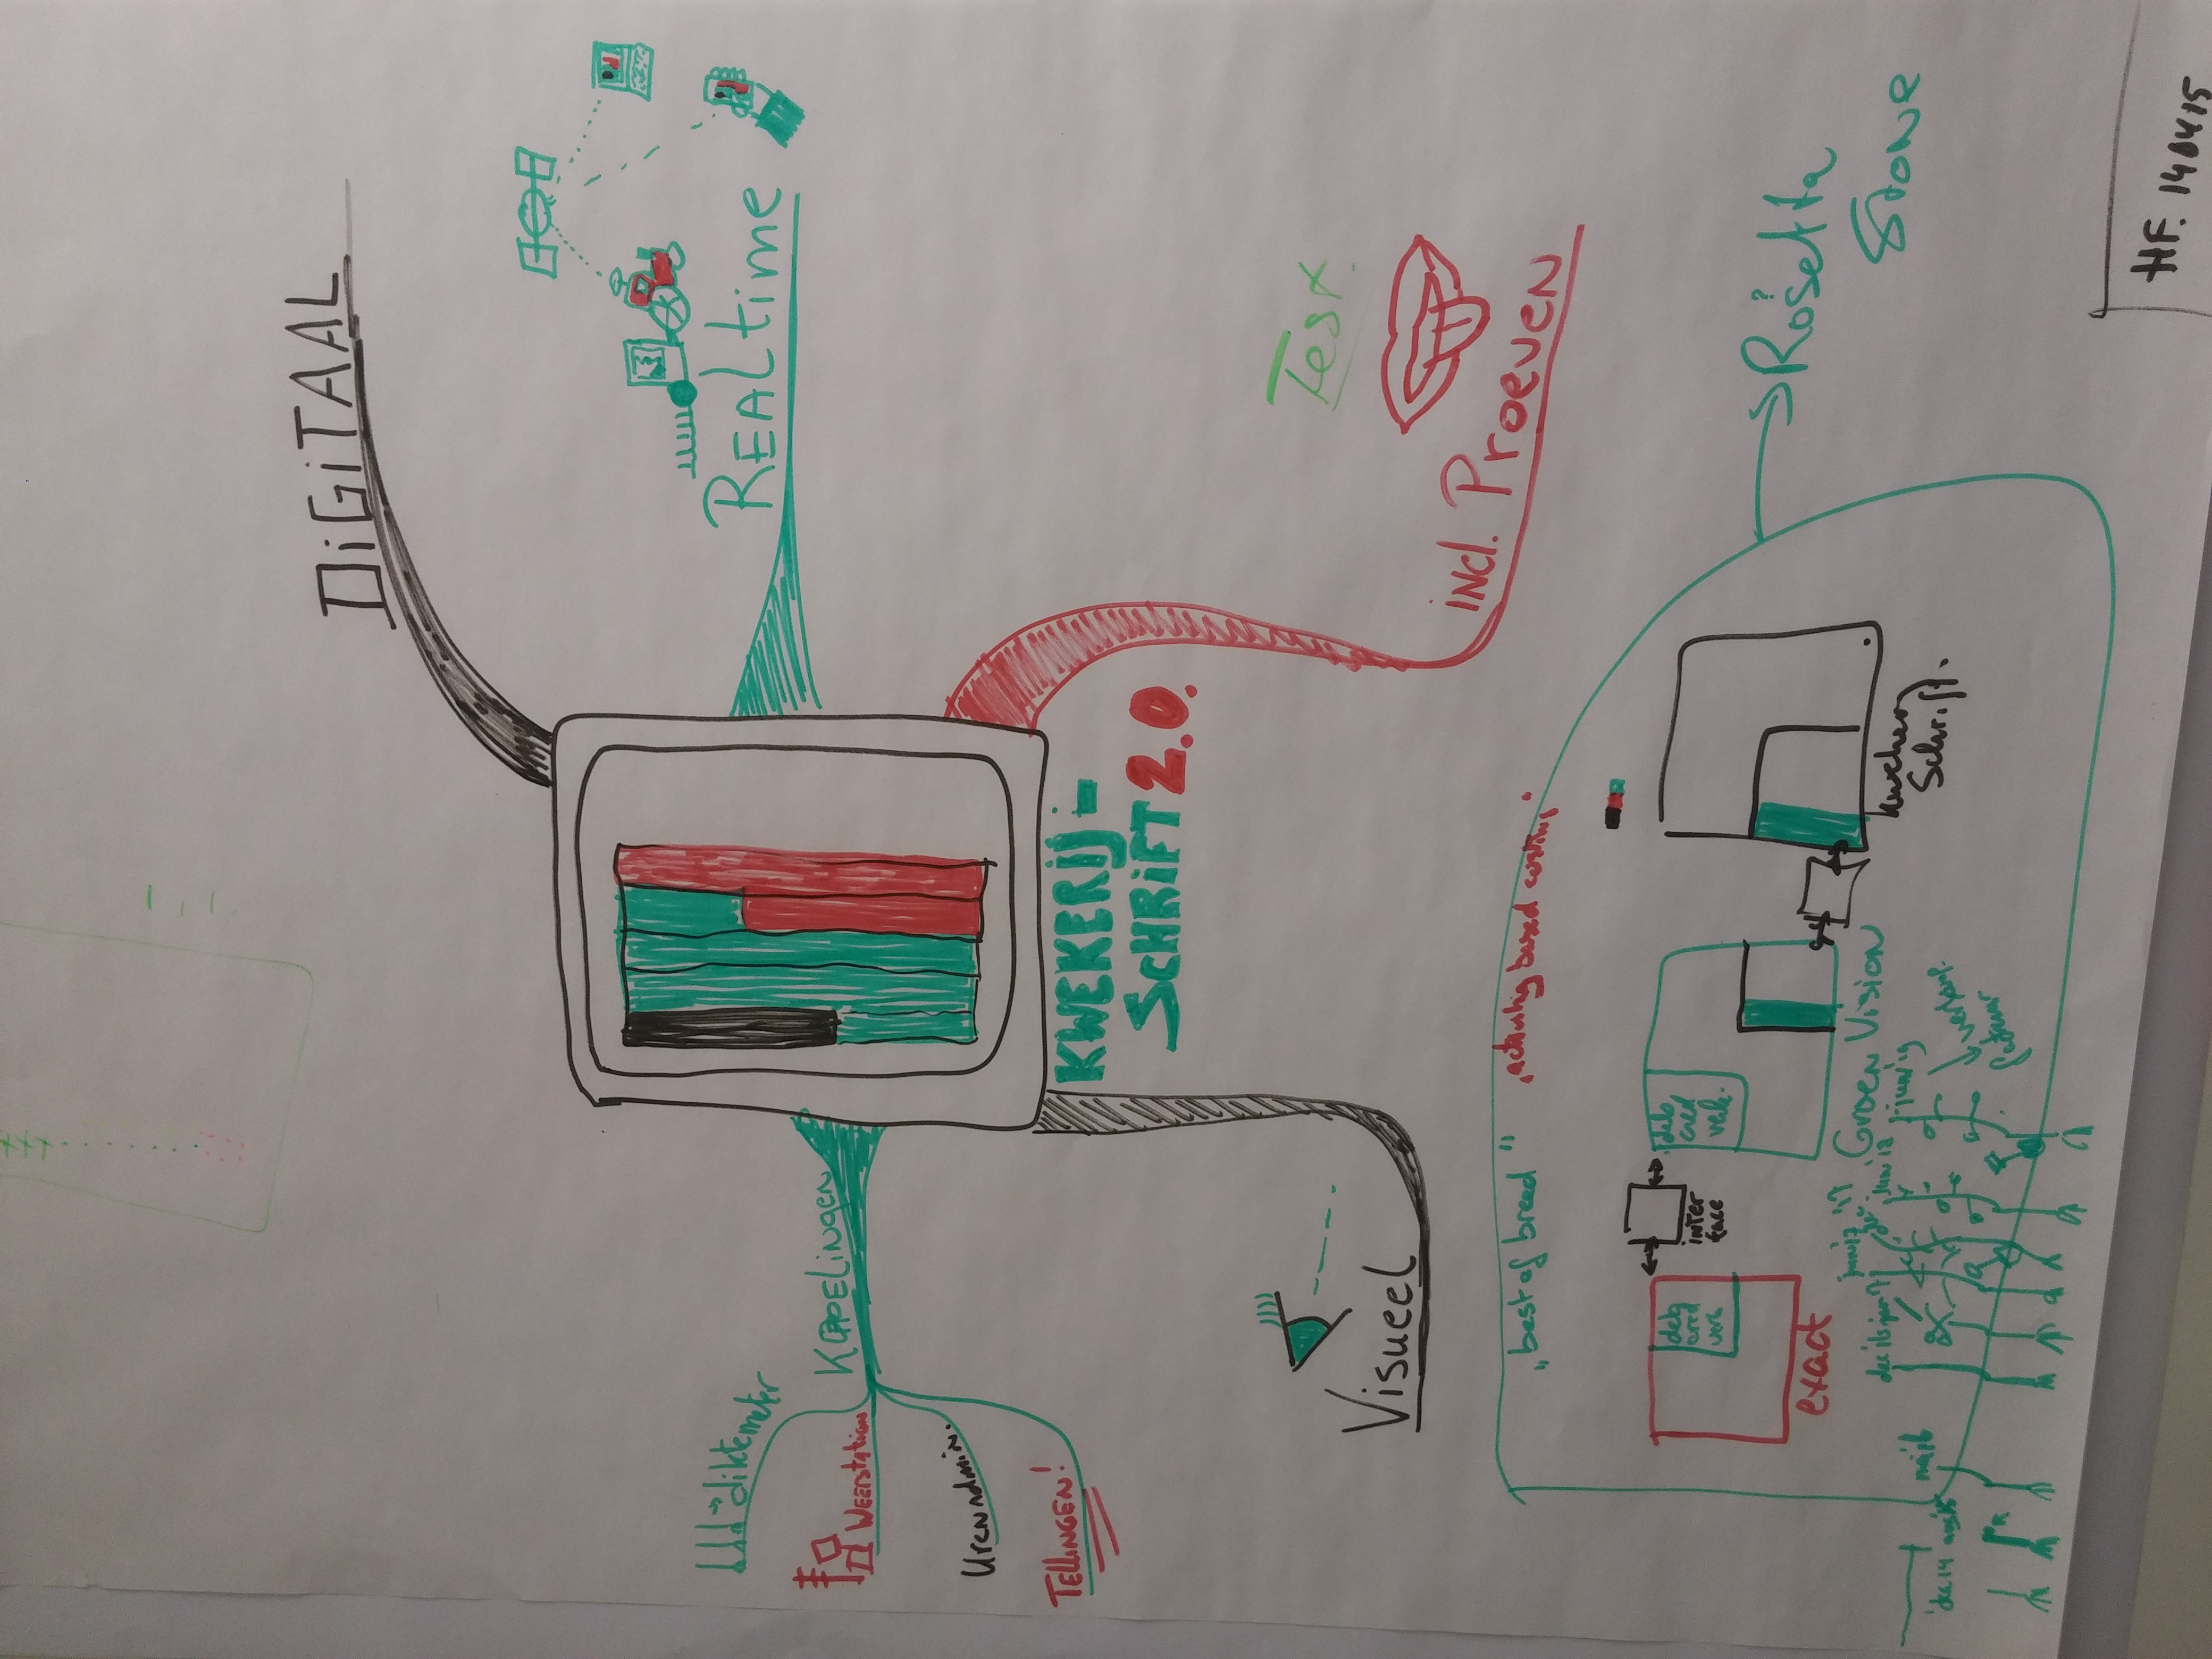
\includegraphics[height=\textwidth, angle=-90]{CustMeeting1.jpg}

\clearpage
\section{Customer meeting (\printdatetitle{17.09.2015})}
\begin{tabular}{ll}
	\textbf{Date:} & \printdate{17.09.2015} \\
	\textbf{Present:} & Jacob van den Boorne, Randy Wilbrink, René, Jan, Martijn, Max \\
	\textbf{Location:} & Reusel \\
\end{tabular}

\textbf{Topics discussed:} \\
How does the system at van den Boorne aardappelen work.

\textbf{Notes:} \\
Jacob is very far with the implementation of precision farming using modern technologies. \\
He can generate overviews of the fields and add different overlays on a map. \\
In the system he can also see weather data and soil scans. \\
The only thing really missing from the Crop-r app is the geocaching. \\
It also turned out that a project plan had already been made by VAA. We asked randy to send it to us.
He can also see pictures which have been taken from the tractor when it was driving down the fields.
Jacob seems to be interested in having  students work for him maybe in a coming sofa?

The system shown by Jacob seems to be the exact thing we are supposed to create during the SoFa.

\clearpage
\section{Customer meeting (\printdatetitle{25.09.2015})}
\begin{tabular}{ll}
	\textbf{Date:} & \printdate{25.09.2015} \\
	\textbf{Present:} & Han Fleuren, Randy Wilbrink, René, Jan, Martijn, Max, Ron \\
	\textbf{Location:} & Fleuren Baarlo \\
\end{tabular}

\textbf{Topics discussed:} \\
How to continue with the project since it already exists for 90\% as crop-r

\textbf{Notes:} \\
The meeting was organised to see how to continue with the project after seeing that Jacob van den Borne was already using an app with almost all the required functionality. \\
We cleared up the possible conflict of interest and asked Randy to provide us with technical information. We also clarified who the customer is and what the goals are for each party participating in the project. And why crop-r is not a problem but more an idea of in which direction our application should go. Further more Han gave some motivational speeches to get the team a bit more focussed.

\clearpage
\section{Customer meeting (\printdatetitle{16.10.2015})}
\begin{tabular}{ll}
	\textbf{Date:} & \printdate{16.10.2015} \\
	\textbf{Present:} & Randy Wilbrink (skype), René, Jan, Martijn, Max, Ron \\
	\textbf{Location:} & Fontys \\
\end{tabular}

\textbf{Topics discussed:} \\
Demo and status update

\textbf{Notes:} \\
Attending Persons \\
*   Randy Wilbrink \\
*   Ron Gebauer \\
*   Jan Kerkenhoff \\
*   Rene Karoff \\
*   Martijn Bonajo \\
*   Max van der Linden 

Agenda \\
*   Show and discuss demo \\
*   Show and discuss mockups \\
*   General feedback \\
*   Whats next? 

Discussion \\
*   There was a discussion about what icons should be used, this however didn't seem to have a high priority. \\
*   When taking a picture on the field the accuracy should be shown and stored. \\
*   When taking a picture on the field the coordinates should be stored. \\
*   Randy pointed out that he was satisfied with the progress so far. \\
*   For the next sprint the focus will be on overlaying fields on the map and finalising the map menu. \\
*   Small meetings like this are more efficient trough Skype since it doesn't involve traveling. 

Action points \\
*   Continue the development of the app with focus on overlaying the fields on the map \\
*   Ask Yannick for GPS data 
\clearpage
\section{Customer meeting (\printdatetitle{24.11.2015})}
\begin{tabular}{ll}
	\textbf{Date:} & \printdate{24.11.2015} \\
	\textbf{Present:} & Yannick Smedts, René, Jan, Martijn, Max, Ron \\
	\textbf{Location:} & Fontys \\
\end{tabular}

\textbf{Topics discussed:} \\
Demo and status update

\textbf{Notes:} \\
Yannick has just returned from Holiday. This meeting is to catch him up with the status of the project. \\
He was really satisfied and surprised with the progress we had made so far.

\clearpage
\section{Customer meeting (\printdatetitle{08.12.2015})}
\begin{tabular}{ll}
	\textbf{Date:} & \printdate{08.12.2015} \\
	\textbf{Present:} & Yannick Smedts (skype), Han Fleuren(skype), Randy Wilbrink (skype) René, Jan, Martijn, Max, Ron \\
	\textbf{Location:} & Fontys \\
\end{tabular}

\textbf{Topics discussed:} \\
Demo and status update

\textbf{Notes:} \\
Show the last touches to the development of the app. //
All stakeholders were very satisfied with the result. //
Received applause from Yannick and Han //
Descision was made to do a 2 week document sprint in stead of 1 because Han, Yannick and Randy were already satisfied with the implementation of the app. \\
Han told us that a golf ball has 320 dimples and weighs 45 grams. \\

\end{document}
